\chapter{Mapping}
\label{cap:mapping}
\thispagestyle{empty}

\begin{quotation}
{\footnotesize
\noindent\emph{Doc: (leggendo) Ho sepolto la DeLorean nella miniera abbandonata di Delgado accanto al vecchio cimitero dei pistoleros mancati come indicato nell'acclusa mappa. Auspicabilmente dovrebbe restare lì indisturbata finché tu non la riporterai alla luce nel 1955. All'interno troverai le istruzioni per ripararla. Il mio alter-ego del 1955 - e cioè io - non dovrebbe avere problemi a ripararla, così tu potrai ritornare al futuro. Quando sarai tornato nel 1985 distruggi la macchina del tempo. Distruggerla? \\
Marty: Sì, beh, è una storia lunga, Doc!}
\begin{flushright}
Ritorno al Futuro, parte III
\end{flushright}
}
\end{quotation}
\vspace{0.5cm}

\section{Introduzione}
Per risolvere il problema della costruzione della mappa si è deciso di utilizzare un approccio basato sulla fusione multisensoriale. Abbiamo deciso di basare l'implementazione del sistema di localizzazione sulla libreria ROAMFREE, Robust Odometry Applying Multisensor Fusion to Reduce Estimation Errors~\cite{conf/icinco/CucciM13}.
Questa libreria gestisce nativamente una grande varietà di sensori, tra cui la IMU e il magnetometro, e si occupa di integrare questi dati per ottenere una odometria robusta. La libreria Inoltre permette di integrare sistemi di estrazione di feature, anche differenti e di stimare la posizione degli oggetti considerati.

Il nostro algoritmo utilizza gli oggetti riconosciuti come punti di rifermento nella mappa e localizza il robot rispetto ad essi. 
Per ottenere questo risultato seguiamo un approccio Full SLAM: viene tenuta traccia di un serie di pose della videocamera e dei punti di riferimento riconosciuti. Da ogni posa del robot è possibile inquadrare un determinato numero di punti di riferimento. Una volta aggiunti una serie di pose e una serie di punti di riferimento, viene ottimizzato simultaneamente l'insieme di pose e la posizione dei punti di riferimento nella mappa, utilizzando il metodo di Gauss-Newton.

Descriveremo nel seguito i dettagli dell'algoritmo utilizzato. Si veda l'\autoref{app:concetti} per i concetti fondamentali necessari alla comprensione dei prossimi paragrafi.


\section{Modello di errore}
Per poter stimare la posizione dei punti di riferimento è necessario definire una misura dell'errore dell'osservazione degli stessi da parte del sistema di estrazione di feature. Il modello usato, trattandosi di una telecamera monoculare, si basa sull'errore di riproiezione della feature nell'immagine.

Abbiamo definito due modelli di errore: uno per analizzare i dati provenienti dal tracker, e un'altro per analizzare i dati provenienti dal riconoscimento ad alto livello.

\subsection{Errore sulle track}
Calcoliamo l'errore sulle track come l'errore di riproiezione del centro di massa della track nell'immagine.
Definiamo la previsione della posizione del centro di massa della track $\hat{z}$ nel seguente modo:

\begin{equation*}
 \hat{z} = \colvec{3}{x}{y}{w} = P\colvec{4}{X}{Y}{Z}{W}
\end{equation*}

Definiamo $\hat{z}'$ come:

\begin{equation*}
 \hat{z}' = \colvec{3}{x/w}{y/w}{1}
\end{equation*}

Sia inoltre $z$ l'osservazione proveniente dal tracker del centro di massa della track considerata, definita come:

\begin{equation*}
 z = \colvec{3}{x_{img}}{y_{img}}{1}
\end{equation*}

Definiamo l'errore di riproiezione come:

\begin{equation*}
 e = \hat{z}' - z + \eta
\end{equation*}

Dove $\eta$ è un rumore bianco gaussiano a media nulla.
La metrica utilizzata per minimizzare l'errore di predizione è quella dei minimi quadrati.

\subsection{Errore sugli oggetti}
La funzione di errore sugli oggetti è più complessa, questo perchè deve tenere traccia delle informazioni semantiche note dell'oggetto, nel nostro caso la forma.

Poichè l'oggetto è formato da un insieme di punti che definiscono la sua forma, definiamo un sistema di coordinate specifico per ciascun oggetto, e chiamiamo $H$ l'isometria che mappa i punti dell'oggetto nei punti dello spazio a tre dimensioni; $H$ definisce quindi la posa dell'oggetto rispetto allo spazio.
Definiamo dunque ogni punto dell'oggetto nel sistema di coordinate dell'oggetto stesso, in modo da poter gestire in maniera semplice le informazioni metriche provenienti dal riconoscimento.
Definiamo la previsione della posizione dell' i-esimo punto dell'oggetto $\hat{z}_i$ nel seguente modo:

\begin{equation*}
 \hat{z}_i =  P\cdot H\cdot\colvec{4}{X}{Y}{Z}{W}
\end{equation*}

Definiamo come nel caso precedente $\hat{z}'$:

\begin{equation*}
 \hat{z}' = \colvec{3}{x/w}{y/w}{1}
\end{equation*}

l'osservazione dell'i-esimo $z_i$ punto è definita come nel caso precedente:

\begin{equation*}
 z = \colvec{3}{x_{img}}{y_{img}}{1}
\end{equation*}

Definiamo l'errore di riproiezione dell'i-esimo punto come:

\begin{equation*}
 e_i = \hat{z}'_i - z_i + \eta
\end{equation*}

Anche in questo caso la metrica utilizzata per minimizzare l'errore di predizione è quella dei minimi quadrati.

\section{Stima}

\begin{figure}[ht]
  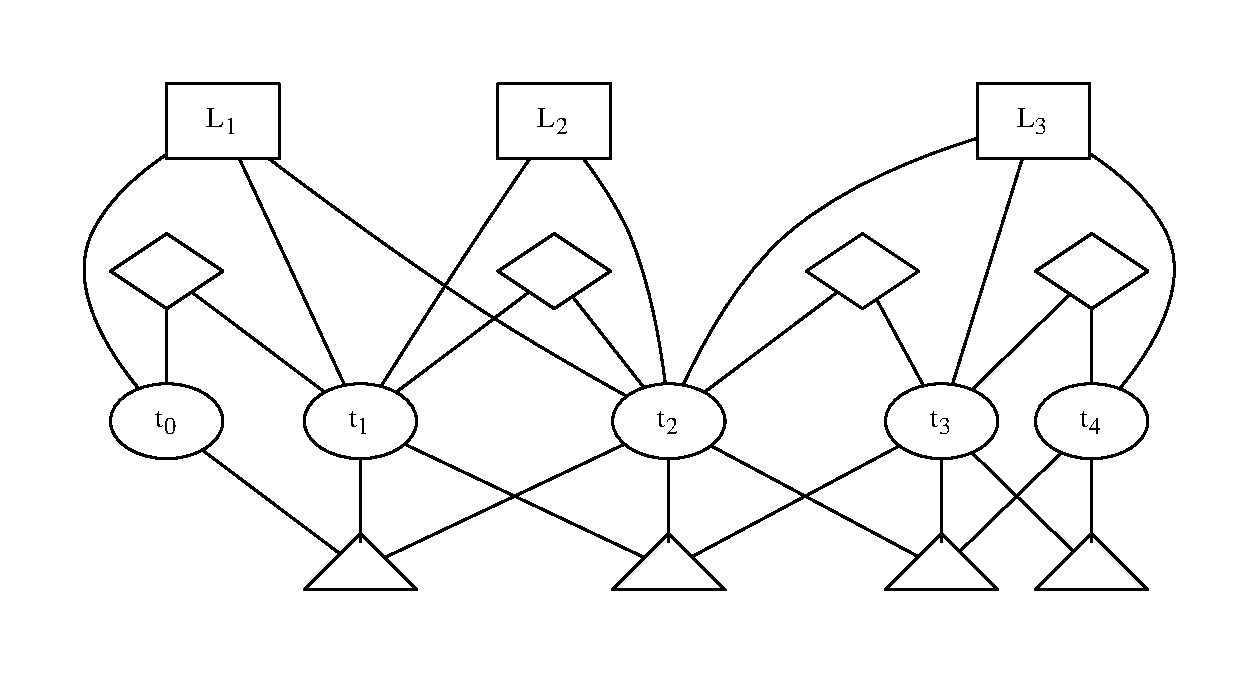
\includegraphics[width=\textwidth]{diagrammi/FactorGraph}
  \caption[Esempio di Factor Graph]{Esempio di un factor graph con nodi che rappresentano le pose (cerchi), e archi che rappresentano i dati della imu (triangoli) e del magnetometro (rombi). Inoltre sono presenti archi rappresentanti i punti di riferimento (quadrati) }
  \label{fig:FactorGraph}
\end{figure}

La stima delle pose della telecamera e della posizione degli oggetti viene fatta tramite un algoritmo batch di bundle adjustment.
Questo algoritmo si basa su tecniche di inferenza Bayesiane, non lineari, sui factor graph che rappresentano la probabilità congiunta delle variabili di stato, date le misure dei sensori e le feature riconosciute.
Il factor graph è un ipergrafo, in cui ogni nodo rappresenta una possibile posa, mentre ogni arco rappresenta un vincolo di misurazione tra due o più ipernodi. Un esempio di factor graph per questo problema è descritto in \autoref{fig:FactorGraph}.

Per calcolare la stima dei parametri, viene lanciato un algoritmo di ottimizzazione basato sul metodo di Gauss-Newton che stimi il massimo a posteriori della distribuzione di probabilità rappresentata dal factor graph, ovvero la configurazione di tutte le variabili di stato che massimizzano la loro probabilità congiunta, date tutte le misure dei sensori e dei punti di riferimento.

Nel caso più semplice, ossia con la sola informazione proveniente dalle track, Le variabili di stato da stimare sono rappresentate semplicemente dal centro di massa delle track, ossia dal centro di massa dei possibili oggetti riconosciuti, e dalla posa della telecamera in ogni istante considerato.

Nel caso di oggetti, le variabili di stato da stimare sono più complesse. Infatti è necessario stimare non solo la posizione relativa dei punti nell'oggetto, ma anche la posa dello stesso, rappresentata dalla matrice $H$; oltre alle pose della telecamera in ogni istante di tempo considerato.


